\section{DINAMICA RELATIVISTICA}

\subsection{Le equazioni della dinamica}

Le equazioni della dinamica newtoniana sono senz'altro accettabili quando le velocità delle particelle sono molto minori della velocità della luce: questo ce lo garantisce l'ottimo accordo fra teoria ed esperienza in moltissime situazioni, dal moto dei pianeti, a quello delle sonde spaziali a quello di cariche lente in campi elettromagnetici, eccetera. Tuttavia, da un lato nulla ci garantisce a priori che le leggi che valgono per basse velocità debbano conservare la loro validità anche nel caso di velocità relativistiche, d'altro lato è evidente che la seconda legge di Newton è in contrasto con il principio di relatività in quanto prevede che una particella possa raggiungere qualsiasi velocità, anche superiore a $c$. Quindi ci troviamo nella necessità di procedere ad una revisione delle leggi della dinamica.\\
Possiamo affrontare il problema in due modi: o indurre le leggi dai fatti sperimentali (come a suo tempo fece Newton), oppure -- con atteggiamento più teorico -- cercare di modificare le leggi di Newton lo stretto necessario in modo da renderle compatibili con il principio di relatività. Seguiremo questa seconda strada che -- deve essere chiaro -- non ha carattere deduttivo (non è possibile dimostrare la necessità delle ipotesi che faremo) per cui, in ultima analisi, la correttezza dei risultati ottenuti può essere sancita esclusivamente dall'accordo con i fatti sperimentali.

I principi della dinamica newtoniana da mettere in discussione sono tre: il primo principio (``un corpo non soggetto a forze o soggetto a forze a risultante nullo si muove di moto rettilineo uniforme'') non contrasta con il principio di relatività in quanto un moto uniforme in un riferimento è uniforme in qualunque altro riferimento, e quindi lo assumiamo vero anche in ambito relativistico. Una volta accettato ne consegue che

\textit{se $\vec F=0$ in un riferimento allora la forza è nulla in qualsiasi altro riferimento \ $(\vec F=0\ \Rightarrow\ \vec F\,'=0)$}

e quindi forze uguali in un riferimento, anche se di natura diversa, sono uguali in ogni riferimento.

Il terzo principio, nella sua formulazione newtoniana (``la forza che A esercita su B è ad ogni istante uguale ed opposta alla forza che B esercita su A''), non può essere vero in generale: A e B possono essere molto lontani e la loro posizione relativa può cambiare nel tempo; il 3$^\circ$ principio richiederebbe che un qualche segnale viaggiasse da un corpo all'altro con velocità infinita: un segnale non è ``puro spirito'' ma qualcosa di molto più concreto, cioè energia e quantità di moto (l'interazione fra due corpi può essere vista come uno scambio di quantità di moto fra di essi), e ciò contrasta con l'esistenza di una velocità limite. Detto in modo diverso, ma equivalente, se in un certo riferimento ad un dato istante le due forze sono uguali (e opposte), questo in generale non è vero in un altro riferimento, in quanto la simultaneità è relativa al riferimento.\\
Anche se il nostro obiettivo è solo quello di costruire la dinamica relativistica per \underline{una} particella, mentre il 3$^\circ$ principio interviene nel caso di sistemi con più particelle, è senz'altro opportuno spendere due parole sia per dare un'idea della profonda revisione dei concetti della meccanica newtoniana, a cominciare dal concetto di forza, che comporta la riformulazione del 3$^\circ$ principio nella meccanica relativistica, sia perché -- come vedremo -- questa revisione influenza anche la formulazione del 2$^\circ$ principio.\\
L'idea newtoniana di azione istantanea a distanza lascia il posto al concetto di campo: l'interazione fra due corpi lontani è sempre mediata (trasmessa) da un campo, il campo elettromagnetico nel caso di particelle cariche, quello gravitazionale fra masse, il campo delle forze nucleari fra i nucleoni, eccetera; ogni particella interagisce ``per contatto'' con il campo, trasferendo ad esso quantità di moto, talvolta anche energia e/o momento della quantità di moto, che viene poi totalmente o parzialmente trasferita, in un tempo finito, all'altra particella. Il campo assume così il ruolo di una vera e propria entità fisica, e quindi è parte del sistema: il sistema delle due particelle non è più un sistema isolato, ma lo è il sistema costituito dalle particelle più il campo (o i campi) con il quale interagiscono. Il 3$^\circ$ principio, che nella fisica newtoniana è equivalente alle leggi di conservazione della quantità di moto e del momento angolare per un sistema isolato, viene nella teoria della relatività sostituito da queste leggi di conservazione per il sistema comprendente anche il campo: è sulla base di queste idee che arriveremo alla formulazione del 2$^\circ$ principio.\\
Si consideri ad esempio l'urto fra due protoni: urto non significa necessariamente contatto fra due sferette dure, ma che le due particelle vengono a trovarsi abbastanza vicine da poter risentire ciascuna delle modifiche del campo dovute all'altra particella (due nucleoni possono interagire tramite il campo delle forze nucleari solo fino ad una distanza che praticamente non supera i $10^{-12}$\,cm); i protoni interagiscono sia con il campo elettromagnetico (sono particelle cariche, e la carica elettrica misura l'intensità dell'interazione con il campo elettromagnetico), sia con quello nucleare: se non tutta l'energia e quantità di moto trasferite dalle particelle ai campi vengono riassorbite dalle particelle, il campo resta ``eccitato'', e questa eccitazione si propaga nello spazio. A questo punto ci mette lo zampino la Meccanica Quantistica, secondo cui le eccitazioni dei campi sono ``quantizzate'', cioè non possono trasportare quantità arbitrarie di energia e quantità di moto, ma solo quantità ben determinate. Ed ecco che nell'urto dei due protoni possono prodursi fotoni, cioè i quanti del campo elettromagnetico, e anche -- se l'energia dei due protoni è sufficientemente elevata -- i mesoni $\pi$, che sono i quanti di eccitazione del campo nucleare.\\
Quindi, in definitiva, nella meccanica relativistica non esiste una vera e propria dinamica dei sistemi nel senso della meccanica newtoniana, cioè sistemi con un numero finito di gradi di libertà, ma la teoria di ogni sistema composto da più particelle interagenti è necessariamente una teoria di campo, e un campo ha infiniti gradi di libertà.

Ma l'obiettivo principale di questo paragrafo è la riscrittura del secondo principio, cioè dell'equazione $\vec F=m\vec a$. Intanto, nella meccanica newtoniana questa equazione può essere scritta come
\begin{equation}
\frac{d\vec p}{dt}=\vec F
\tag{5.1}
\end{equation}
dove con $\vec p$ abbiamo indicato la quantità di moto della particella. Conformemente al nostro programma di modificare la (5.1) lo stretto necessario per renderla compatibile con il principio di relatività, vediamo quali concetti fondamentali della meccanica newtoniana possono sopravvivere in una formulazione relativistica: la forza $\vec F$ a secondo membro della (5.1) è il risultato dell'interazione della particella con un altro sistema e, se $\vec P$ è la sua quantità di moto, si ha
\begin{equation}
\frac{d\vec P}{dt}=-\vec F\quad\ \Rightarrow\quad\ \frac{d\vec p}{dt}=-\frac{d\vec P}{dt}\,\cdot
\tag{5.2}
\end{equation}
La (5.2) esprime la conservazione della quantità di moto per il sistema costituito dalla particella e l'esterno con cui interagisce, e permette di ridefinire la forza come la quantità di moto trasferita alla particella (dall'esterno) nell'unità di tempo (definizione dinamica di forza). Questa definizione può essere adottata tale quale anche in ambito relativistico in quanto, come abbiamo visto nella discussione precedente, la conservazione della quantità di moto totale del sistema particella--esterno (campo, \dots) viene assunta come formulazione del 3$^\circ$ principio nella meccanica relativistica. Quindi la (5.1) è anche -- per definizione di forza -- l'equazione del moto relativistica per una particella: il problema è spostato sulla definizione di $\vec p$, che non può mantenere la forma newtoniana $\vec p=m\vec v$. Assumeremo che la quantità di moto di una particella abbia la forma
\begin{equation}
\vec p=f(v)\vec v;\qquad\quad f(0)=m
\tag{5.3}
\end{equation}
cioè che $\vec p$ sia proporzionale a $\vec v$, con coefficiente di proporzionalità che dipende solo dal modulo della velocità (in uno spazio omogeneo ed isotropo esistono forse alternative?) e cercheremo di determinare $f(v)$ assumendo la conservazione della quantità di moto in ogni riferimento per il sistema costituito dalla particella e da ciò con cui interagisce.\\
Possiamo anche scrivere, poiché ci sarà utile, la (5.3) in termini della quadrivelocità $\vec u\equiv\gamma(v)\vec v$:
\begin{equation}
\vec p=g(v)\vec u,\quad g(0)=m\qquad\quad\Big(g(v)=f(v)/\gamma(v)\Big).
\tag{5.4}
\end{equation}
Consideriamo l'urto fra due particelle 1 e 2 di uguale massa, che in un riferimento $K_0$ hanno inizialmente velocità uguali e opposte $\vec v$ e $-\vec v$ (figura 5.1a); assumiamo che l'urto avvenga per contatto, o che comunque il campo che trasmette l'interazione non resti eccitato, per cui la quantità di moto prima e dopo l'urto è solo quella delle due particelle. Inoltre assumiamo che l'urto sia elastico, cioè con conservazione dell'energia cinetica totale. Non conosciamo ancora l'espressione dell'energia cinetica (relativistica) di una particella, ma ci basta supporre che sia una funzione crescente della velocità $E(v)$. La conservazione della quantità di moto, sia che si utilizzi l'espressione (5.3) o la (5.4), ci permette di concludere (basta assumere che $f(v)v$ sia una funzione iniettiva) che dopo l'urto le due particelle hanno velocità uguali ed opposte e dalla conservazione dell'energia si deduce che il modulo delle velocità è ancora $v$.
\begin{center}
\begin{tabular}{cc}
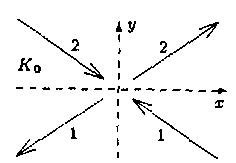
\includegraphics[scale=1.2]{fig/fig5_1a} & 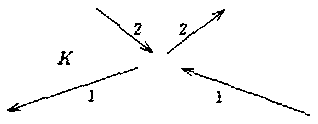
\includegraphics[scale=1.2]{fig/fig5_1b}\\
{\small fig.~5.1a} & {\small fig.~5.1b}
\end{tabular}
\end{center}
Prendiamo gli assi $x$ e $y$ come in figura 5.1a, per cui le componenti $x$ delle velocità di ciascuna delle due particelle sono uguali prima e dopo l'urto, e le componenti $y$ cambiano segno. Osserviamo ora il processo da un riferimento $K$ in moto rispetto a $K_0$ in direzione dell'asse $x$ (figura 5.1b): per le (4.66) anche in $K$ le componenti $x$ delle velocità di ciascuna delle due particelle sono uguali prima e dopo l'urto, e le componenti $y$ cambiano segno, pertanto la stessa cosa vale anche per le quadrivelocità, il cui modulo quindi non cambia nell'urto. Inoltre, grazie alle (4.71), le componenti $y$ delle quadrivelocità delle due particelle sono uguali fra di loro (a parte il segno), in quanto sono uguali nel riferimento $K_0$:
\begin{equation}
|u_{1,y}|=|u_{2,y}|
\tag{5.5}
\end{equation}
(mentre invece dalle (4.66) si vede che le componenti $y$ delle velocità delle due particelle sono diverse). Per la conservazione della quantità di moto in $K$, utilizzando la (5.4) e la (5.5) si ha ($\Delta\vec p$, $\Delta\vec u$ rappresentano le variazioni nell'urto e sono dovute soltanto al cambiamento di direzione di $\vec p$ e di $\vec u$)
\begin{equation}
\begin{aligned}
&|\Delta\vec p_1|=g(v_1)\,|\Delta\vec u_1|=2g(v_1)\,|u_{1,y}|;\quad\ |\Delta\vec p_2|=2g(v_2)\,|u_{2,y}|=2g(v_2)\,|u_{1,y}|\\
&\Delta\vec p_1+\Delta\vec p_2=0\ \Rightarrow\ |\Delta\vec p_1|=|\Delta\vec p_2|\ \Rightarrow\ g(v_1)=g(v_2)
\end{aligned}
\tag{5.6}
\end{equation}
L'arbitrarietà della velocità di $K$ rispetto a $K_0$ e della velocità $v$ delle due particelle in $K_0$ permettono di concludere che $v_1$ e $v_2$ sono indipendenti, e quindi che $g$ è indipendente da $v$. Dalla (5.4) si ha allora $g=m$, cioè
\begin{equation}
\vec p=m\vec u=m\gamma(v)\,\vec v
\tag{5.7}
\end{equation}
che è l'espressione relativistica della quantità di moto.

\paragraph{Esempi}
\begin{enumerate}
\item Studiamo il moto unidimensionale di una particella soggetta ad una forza costante $F$.\\
Dalla (5.1) e (5.7), posto $g\equiv F/m$ e presi $v(0)=0$, \ $x(0)=0$, si ha
\begin{equation}
\begin{aligned}
&\frac{v}{\sqrt{1-v^2/c^2}}=gt\quad\ \Rightarrow\quad\ v(t)=\frac{gt}{\sqrt{1+(gt/c)^2}}\quad\ \Rightarrow\\
&x(t)=\frac{c^2}{g}\left(\sqrt{1+(gt/c)^2}-1\right)
\end{aligned}
\tag{5.8}
\end{equation}
o anche
\begin{equation}
\big(x+c^2/g\big)^2-c^2t^2=\big(c^2/g\big)^2
\tag{5.9}
\end{equation}
e quindi la linea di universo della particella è un'iperbole (e pertanto questo è detto ``moto iperbolico'').\\
Per $|t|\ll c/g$ \ (se $g$ è l'accelerazione di gravità \ $c/g=3\times10^7$\,s, cioè $\approx1$\,anno) si ritrovano le leggi del moto uniformemente accelerato.
\item Moto bidimensionale di una particella carica in un campo magnetico uniforme.\\
La forza (di Lorentz) è sempre ortogonale alla velocità e quindi anche alla quantità di moto, per cui può cambiare solo la direzione (e non il modulo) di $\vec p$, e quindi di $\vec v$. Allora
\begin{equation}
\frac{d\vec p}{dt}=m\,\gamma(v)\frac{d\vec v}{dt}=q\frac{\vec v}{c}\wedge\vec B
\tag{5.10}
\end{equation}
per cui, essendo $\gamma(v)$ costante, la soluzione coincide con quella non relativistica pur di sostituire $m$ con $m\,\gamma(v)$: la particella descrive una circonferenza di raggio $\rho$ con velocità angolare $\omega$ dati da
\begin{equation}
\rho=\frac{p\,c}{qB},\qquad\quad\omega=\frac{qB}{m\,\gamma(v)c}\,\cdot
\tag{5.11}
\end{equation}
\end{enumerate}

\subsection{L'energia}

Nella meccanica non relativistica la definizione di energia cinetica nasce dal teorema delle forze vive, per cui tentiamo la stessa strada anche in ambito relativistico; dalla (5.1)
\begin{equation}
\frac{d\vec p}{dt}\cdot\vec v=\vec F\cdot\vec v
\tag{5.12}
\end{equation}
ed ora si ha si tratta di vedere se il 1$^\circ$ membro può essere scritto come la derivata di una funzione $E(v)$. Siccome
\begin{equation}
\frac{d\,\gamma(v)}{dt}=\frac{1}{c^2}\gamma^3\,\vec v\cdot\frac{d\vec v}{dt}
\tag{5.13}
\end{equation}
si ha
\begin{equation}
\frac{d\vec p}{dt}\cdot\vec v=m\vec v\cdot\frac{d\vec v}{dt}\left(\frac{v^2}{c^2}\gamma^3+\gamma\right)=m\gamma^3\,\vec v\cdot\frac{d\vec v}{dt}=mc^2\frac{d\,\gamma(v)}{dt}
\tag{5.14}
\end{equation}
quindi definita l'\textbf{energia}
\begin{equation}
E(v)\defeq m\gamma(v)c^2
\tag{5.15}
\end{equation}
abbiamo il \textbf{teorema delle forze vive} nella forma
\begin{equation}
\frac{dE(v)}{dt}=\vec F\cdot\vec v\,.
\tag{5.16}
\end{equation}
Per piccole velocità dalla (4.41) abbiamo
\begin{equation}
E(v)=mc^2+\frac{1}{2}mv^2+O(v^4/c^4)
\tag{5.17}
\end{equation}
quindi $E(v)$ differisce (per piccole velocità) dall'energia cinetica non relativistica per la costante $mc^2$: ciò non costituisce un problema in quanto nel teorema delle forze vive intervengono sempre e soltanto differenze di energia. Si potrebbe ridefinire l'energia (cinetica) sottraendo $mc^2$ ad $E(v)$, tuttavia ciò non conviene per la seguente ragione: se osserviamo la definizione della quadrivelocità data dalla (4.69), si riconosce che
\begin{equation}
\frac{E(v)}{c}=mu_0
\tag{5.18}
\end{equation}
quindi possiamo definire il \textbf{quadrivettore energia--quantità di moto}
\begin{equation}
p\defeq mu\equiv\Big(p_0=\frac{E}{c},\ \vec p\,\Big)=\big(mc\gamma(v),\ m\gamma(v)\vec v\,\big)
\tag{5.19}
\end{equation}
le cui leggi di trasformazione sono identiche a quelle della quadrivelocità e quindi a quelle delle coordinate: per trasformazioni senza rotazioni
\begin{equation}
\left\{\begin{aligned}
E'&=\gamma(v)(E-v\,p_x)\\
p_x'&=\gamma(v)\Big(p_x-v\frac{E}{c^2}\Big)\\
p_y'&=p_y\\
p_z'&=p_z\,.
\end{aligned}\right.
\tag{5.20}
\end{equation}
L'invariante (per trasformazioni di Lorentz) associato al quadrivettore $p$ è
\begin{equation}
(p,p)={}^tp\,G\,p=-\frac{E^2}{c^2}+\vec p\,^2=-m^2c^2\gamma^2\,(1-v^2/c^2)=-m^2c^2.
\tag{5.21}
\end{equation}
Dalla (5.19) e dalla (5.21) si ha
\begin{equation}
\vec v=c^2\,\frac{\vec p}{E};\qquad\qquad E=\sqrt{\vec p\,^2c^2+m^2c^4}\,.
\tag{5.22}
\end{equation}
Nella meccanica relativistica i concetti di quantità di moto e di energia sono ``primitivi'' rispetto al concetto di velocità, una delle ragioni è che nelle equazioni del moto interviene la quantità di moto e non (direttamente) la velocità, un'altra è di carattere più sperimentale: la velocità non può superare la velocità della luce, mentre quantità di moto ed energia non sono limitate superiormente; non è certo facile distinguere (sperimentalmente) una velocità di $0.99c$ da una di $0.999c$, mentre il fattore $\gamma(v)$, che entra sia nella definizione della quantità di moto che dell'energia, in un caso vale (circa) 7.1, e nell'altro 22.4.\\
Ma la ragione più importante sta nel fatto che in natura esistono particelle di massa nulla: i fotoni (quanti di luce) e (forse) i neutrini. In questi casi quantità di moto ed energia non sono definiti dalle (5.7) e (5.15), ma sono grandezze primitive, legate fra di loro dal fatto che l'invariante $(p,p)$ è nullo e quindi \ $E=c|\vec p\,|$; \ $p$ è un quadrivettore di tipo luce e non esiste il riferimento tangente alla particella, cioè un riferimento in cui $\vec p=0$: dalla (5.22) segue infatti che la velocità di queste particelle è $c$ in qualsiasi riferimento.

\subsection{Massa ed energia}

La teoria della relatività di Einstein costituisce una delle rivoluzioni scientifiche di questo secolo, e come tale ha attratto l'attenzione anche dei ``non addetti ai lavori'', come filosofi, storici ed anche, in buona misura, dell'uomo della strada. Se fate una piccola indagine in questi ambienti di non addetti ai lavori (ma non solo), scoprirete che ai primi posti di quelli che sono considerati i punti di rottura più rilevanti rispetto alla fisica newtoniana, viene citata la dipendenza della massa dalla velocità. Eppure fino a questo punto questo concetto qui non è venuto fuori! La ragione sta nel fatto che fra gli addetti ai lavori esistono due scuole di pensiero (e nemmeno tanto tolleranti l'una nei riguardi dell'altra): una, e corrisponde al punto di vista che noi abbiamo adottato, definisce la massa come un invariante, e pertanto indipendente dalla velocità, l'altra definisce la massa come $m=m_0\gamma(v)$, dove $m_0$ è la ``massa a riposo'', cioè quella che per noi è tout--court la massa (invariante). Questo secondo punto di vista corrisponde a chiedersi come deve essere modificata la definizione della massa affinché la (5.1) sia compatibile con il principio di relatività, mentre noi ci siamo chiesti come deve essere modificata la definizione di quantità di moto. È chiaro che le definizioni non cambiano la fisica, e quindi non c'è nulla di sbagliato nell'adottare una o l'altra definizione di massa, ma è lecito chiedersi quale sia più opportuna. La scuola pisana appartiene alla prima scuola di pensiero, e quindi è scontato che qui metteremo in evidenza i pregi della prima definizione ed i difetti della seconda. In primo luogo, qualunque fisico sperimentale delle alte energie quando produce una nuova particella ne misura l'energia e la quantità di moto e determina la sua massa tramite la (5.21), che fornisce la massa invariante; in secondo luogo, la cosiddetta massa relativistica altro non è, a parte il fattore costante $c^2$, che l'energia: che ragione c'è per chiamare con nomi diversi la stessa cosa? Un illustre fisico sostiene che molte delle discussioni fra i fisici nascono dal fatto che chiamano con lo stesso nome cose diverse, e con nomi diversi la stessa cosa. Ammesso che i sostenitori della massa relativistica siano d'accordo su quanto sopra, a questo punto tirano fuori l'asso dalla manica: tutto bene, però è inconfutabile, data l'esistenza di una velocità limite, che l'inerzia (forza/accelerazione\,?) aumenta con la velocità. È vero, se però nella (5.1) esplicitiamo la dipendenza dall'accelerazione, ci accorgiamo che i coefficienti dell'accelerazione tangenziale e di quella normale sono diversi, e sono dati rispettivamente da $m\gamma^3$ e da $m\gamma$ (il primo lo abbiamo trovato nella derivazione del teorema delle forze vive, il secondo nel moto di una carica in campo magnetico), e quindi se vogliamo identificare l'inerzia con la massa relativistica dovremmo introdurre due masse, una longitudinale ed una trasversale.

Ma allora la famosa e celebrata equivalenza massa--energia dove va a finire? Questo è un problema diverso, ed è un problema serio, non di definizioni. Va un po' oltre gli scopi di questa introduzione alla teoria della relatività una discussione esauriente di questo problema, che riguarda la dinamica dei sistemi composti, tuttavia data la sua rilevanza cercheremo di mettere a fuoco, anche se solo su un esempio, i concetti fondamentali.\\
Consideriamo un sistema di due particelle 1 e 2 che effettuano un urto; supponiamo che le particelle interagiscano solo a piccole distanze, per cui prima dell'urto possono essere considerate particelle libere. La quantità di moto prima dell'urto è
\begin{equation}
\vec P=\vec p_1+\vec p_2
\tag{5.23}
\end{equation}
e siccome si conserva tale è anche dopo l'urto: per esempio, se le particelle dopo l'urto sono libere (cioè non sono rimaste attaccate) e il campo che trasmette l'interazione non si porta via quantità di moto allora
\begin{equation}
\vec p_1\,'+\vec p_2\,'=\vec P\,.
\tag{5.24}
\end{equation}
Si ha il seguente fondamentale

\textbf{\textit{Teorema:}} \textit{se la quantità di moto si conserva in tutti i riferimenti, allora si conserva (in tutti i riferimenti) anche l'energia.}

Infatti, posto \ $\vec P=\vec p_1+\vec p_2$, \ $E=E_1+E_2$, \ dette \ $\Delta\vec P$, $\Delta E$ \ le loro variazioni nell'urto, se $K$ e $K'$ sono due riferimenti dalla seconda delle (5.20) si ha
\begin{equation}
0=\Delta P_x'=\gamma(v)\Big(\Delta P_x-v\frac{\Delta E}{c^2}\Big)=-\gamma(v)v\frac{\Delta E}{c^2}\quad\ \Rightarrow\quad\ \Delta E=0
\tag{5.25}
\end{equation}
e poi dalla prima delle (5.20) segue \ $\Delta E'=0$. \ $\blacksquare$\\
Il teorema appena dimostrato ha validità generale; esso si applica ad ogni sistema isolato, qualunque sia la sua natura: un nucleo, costituito da nucleoni e campo delle forze nucleari; un atomo, costituito da un nucleo, elettroni e campo elettrico, \dots\,.\\
Il teorema richiede solo che per il sistema sia definita la quantità di moto (totale) $\vec P$ e l'energia $E$, e che questi si trasformino come un quadrivettore: allora, siccome per il 3$^\circ$ principio la quantità di moto si conserva, e per il principio di relatività ciò è vero in ogni riferimento, ne segue che anche l'energia si conserva.

Ritorniamo alle nostre particelle che si urtano: da quanto sopra segue che nel processo d'urto che stiamo considerando si conserva anche l'energia.\\
Ma allora esistono solo gli urti elastici? E se le due particelle restano attaccate? Esaminiamo la situazione. Supponiamo per semplicità che le due particelle abbiano la stessa massa $m$, che inizialmente viaggino con velocità opposte $\vec v$ e $-\vec v$ sulla stessa retta, e che dopo l'urto restino attaccate. Prima dell'urto la quantità di moto totale $\vec P$ è nulla, l'energia è
\begin{equation}
E=E_1+E_2=2m\gamma(v)c^2
\tag{5.26}
\end{equation}
e siccome si conservano queste sono anche la quantità di moto e l'energia della particella composta che si forma nell'urto e quindi, per la (5.21), la particella composta ha una massa data da
\begin{equation}
M^2c^4=E^2-\vec P\,^2c^2=(E_1+E_2)^2-0\quad\ \Rightarrow\quad\ M=2m\gamma(v)>2m
\tag{5.27}
\end{equation}
In altri termini, la conservazione dell'energia e della quantità di moto implica la non conservazione (o la non additività) della massa.\\
Ma l'urto è anelastico e l'energia si conserva: ne segue che l'energia cinetica nel riferimento del centro di massa, nel nostro caso data da
\begin{equation}
E_1+E_2-2mc^2=2\big(\tfrac{1}{2}mv^2+\cdots\big)
\tag{5.28}
\end{equation}
si converte in altra forma di energia (legge generale di conservazione dell'energia o 1$^\circ$ principio della termodinamica): energia interna (e quindi la particella composta è più calda dei componenti prima dell'urto), oppure energia potenziale (p.es.\ fra le due particelle poteva esserci una molla che poi resta bloccata alla massima compressione), eccetera: la massa $M$ della particella composta, moltiplicata per $c^2$, è uguale quindi a tutto il contenuto energetico della particella, non solo alla somma delle energie di riposo ($2mc^2$) dei componenti, ma anche a tutte le altre forme di energia \underline{interna} (cioè nel riferimento in cui il sistema ha quantità di moto nulla) al sistema: questo è il significato dell'equivalenza massa--energia o, equivalentemente, del termine ``inerzia dell'energia''.\\
Nel caso di un gas, per esempio, o di qualsiasi altro sistema termodinamico, $Mc^2$ eguaglia quindi, a meno di una costante $(\sum_im_ic^2)$, l'energia interna $\mathcal U$ del sistema.

Qualsiasi sistema composto, sia esso un sistema ``compatto'' (come un nucleo, un atomo e -- chi lo sa? -- forse un elettrone, un protone \dots), o anche un insieme di particelle indipendenti, è quindi caratterizzato \underline{esternamente} da una massa che coincide, a parte il fattore $c^2$, con l'energia totale del sistema nel riferimento del centro di massa (riferimento in cui $\vec P=0$), la cui origine risiede quindi, almeno in parte, nella struttura interna del sistema.\\
Così, per esempio, il deutone (nucleo del deuterio, isotopo dell'idrogeno con numero atomico $A=2$) è una particella composta da un protone e un neutrone tenuti insieme dalle forze nucleari, e la sua massa è inferiore di 2.2\,MeV$/c^2$ alla somma delle masse dei componenti (1\,MeV $=10^6$\,eV\,; protone e neutrone hanno masse quasi uguali e di circa 940\,MeV$/c^2$); questo \textbf{difetto di massa} (che si ha per tutti i nuclei) è dovuto al fatto che, poiché il sistema è legato (cioè occorre fornirgli energia per dissociarlo), il contributo dell'energia potenziale è negativo.\\
Nella \textbf{fusione} di due nuclei i prodotti della reazione hanno massa inferiore alla somma delle masse dei componenti, per cui si libera energia: consideriamo p.es.\ la fusione di deuterio e trizio (nucleo dell'isotopo dell'idrogeno con $A=3$) che produce una particella $\alpha$ (nucleo dell'atomo di elio) ed un neutrone
\begin{equation}
d+t\to\alpha+n\,.
\tag{5.29}
\end{equation}
Siccome deuterio e trizio sono (praticamente) in quiete, si ha
\begin{equation}
E^i=M_dc^2+M_tc^2=E^f=M_\alpha\gamma(v_\alpha)c^2+M_n\gamma(v_n)c^2
\tag{5.30}
\end{equation}
e l'energia liberata (sotto forma di energia cinetica dei prodotti della reazione) è data da
\begin{equation}
\begin{aligned}
&M_\alpha\big(\gamma(v_\alpha)-1\big)c^2+M_n\big(\gamma(v_n)-1\big)c^2=(M_d+M_t-M_\alpha-M_n)\,c^2\\
&\quad=17.6\,\mathrm{MeV}
\end{aligned}
\tag{5.31}
\end{equation}
(a questo punto è chiaro perché è consuetudine esprimere le masse delle particelle e dei nuclei in MeV$/c^2$, e anche in GeV$/c^2$: \ 1\,GeV $=10^9$\,eV\,).\\
Il problema della fusione consiste principalmente nel fatto che per realizzare la reazione occorre portare i nuclei ad una distanza $d$ dell'ordine di $10^{-12}$\,cm, ma fra i nuclei si esercita la repulsione coulombiana, per cui è necessario che essi abbiano un'energia cinetica dell'ordine di $e^2/d\approx10^5$\,eV, e quindi che il plasma (gas di nuclei ed elettroni: alla temperatura che stiamo per determinare gli atomi sono completamente ionizzati) abbia una temperatura $T\approx10^9$\,K: non secondario è il problema di riscaldare il plasma, mantenendolo confinato in una regione lontana dalle pareti del contenitore.

\subsection{La legge di trasformazione delle forze}

La legge di trasformazione della forza è definita dal fatto che la (5.1) deve essere soddisfatta in ogni riferimento e quindi è identica a quella di \ $d\vec p/dt$; anche la legge di trasformazione della forza, come quella della velocità, è abbastanza complicata, e la ragione è la stessa: si trasformano sia il numeratore ($\Delta\vec p$) che il denominatore ($\Delta t$). Nel caso della velocità abbiamo trovato utile introdurre la quadrivelocità, qui conviene introdurre la \textbf{quadriforza} $G=(G_0,\,\vec G)$
\begin{equation}
G\defeq\frac{dp}{d\tau}=\Big(\frac{dp_0}{d\tau},\ \frac{d\vec p}{d\tau}\Big)
\tag{5.32}
\end{equation}
come la derivata del quadrivettore energia--quantità di moto rispetto al tempo proprio, per cui -- se $\vec v$ è la velocità della particella -- grazie alla (4.67) e alla (5.16) (teorema delle forze vive)
\begin{equation}
G_0=\frac{\gamma(v)}{c}\vec F\cdot\vec v;\qquad\vec G=\gamma(v)\vec F\,.
\tag{5.33}
\end{equation}
Per cambiamenti di riferimento la quadriforza, come la quadrivelocità, si trasforma come ogni quadrivettore (coordinate spazio-temporali, energia--quantità di moto \dots): se $\vec u$ (in direzione degli assi $x$, come al solito) è la velocità di $K'$ rispetto a $K$,
\begin{equation}
\left\{\begin{aligned}
\gamma(v')F_x'&=\gamma(u)\Big(\gamma(v)F_x-\frac{u}{c}\frac{\gamma(v)}{c}\vec F\cdot\vec v\Big)\\
\gamma(v')F_y'&=\gamma(v)F_y\\
\gamma(v')F_z'&=\gamma(v)F_z
\end{aligned}\right.
\qquad\qquad\vec v\,'=\vec v\circ(-\vec u).
\tag{5.34}
\end{equation}
In particolare, se $\vec v$ è la velocità della particella nel riferimento del laboratorio, $\vec F^0$ la forza nel suo riferimento di quiete istantanea e \ $G^0=(0,\,\vec F^0)$ \ la quadriforza e gli assi $x$ del riferimento tangente e di quello del laboratorio coincidono con la direzione di $\vec v$, si ha
\begin{equation}
\begin{aligned}
&G_x\equiv\gamma(v)F_x=\gamma(v)(G_x^0+0)&&\Rightarrow\quad F_x=F_x^0\\
&G_y\equiv\gamma(v)F_y=G_y^0=F_y^0&&\Rightarrow\quad F_y=\frac{1}{\gamma(v)}F_y^0\\
&\quad\dots
\end{aligned}
\tag{5.35}
\end{equation}
quindi la componente $x$ della forza, che è la componente nella direzione di $\vec v$ (``componente longitudinale'' $F_\parallel$), resta invariata passando dal riferimento tangente al laboratorio, e quindi è uguale in tutti i riferimenti, mentre la componente della forza ortogonale a $\vec v$ (``componente trasversa'' $F_\perp$) si riduce del fattore $\gamma(v)$ rispetto al suo valore nel riferimento tangente:
\begin{equation}
F_\parallel=F_\parallel^0\,;\quad\ F_\perp=\frac{1}{\gamma(v)}F_\perp^0\,.
\tag{5.36}
\end{equation}
